\section{Pianificazione dei test}

Si vuole adottare una strategia di verifica del software tramite test opportunamente predeterminati e che garantiscano almeno un test per ogni requisito. I test sono l'applicazione delle tecniche di verifica dinamica introdotte nelle \NormeDiProgetto{}; tali attività, oltre a richiedere l'esecuzione del programma, devono poter essere ripetibili, ossia tramite delle specifiche su come riprodurre i test vogliamo che il loro output sia deterministico. \`E importante che i test di unità vengano svolti in parallelo, dando precedenza alle unità che producono risultati utili alla comprensione del loro funzionamento integrato, l'ambiente di testing deve soddisfare tale obiettivo. \\
L'attività di test deve produrre un \glossario{log} che specifica quando e chi ha eseguito il test e con quali input; l'insorgenza di \glossario{failure} deve essere tracciata e catalogata.

	\subsection{Livelli di testing}
	Il testing del software viene suddiviso in livelli differenti e si concretizzano in un esecuzione bottom-up che avanza sequenzialmente alle attività di codifica e  di validazione. 
	I test che si andranno ad applicare sono di cinque tipi, riservando la specifica delle ultime due tipologie alla prossima revisione:

	\begin{enumerate}
		\item Test di Validazione (TV): viene verificato che il prodotto soddisfi quanto richiesto dal \glossario{proponente} individuando delle macro azioni da eseguire sul sistema che un normale utente svolge comunemente;
		\item Test di Sistema (TS): sono test relativi al comportamento dell'intero sistema ossia viene verificato che la sua architettura generale funziona complessivamente bene;
		\item Test di Integrazione (TI): vengono verificate le componenti del sistema contenute nella \SpecificaTecnica{}, ossia viene verificato che i \glossario{package} siano funzionanti e in grado di funzionare nel loro insieme; %PACKAGE
		\item Test di Unità (TU): viene testata ogni unità, ossia la più piccola parte di lavoro assegnabile ad un programmatore. In questo progetto una unità dovrebbe corrispondere ad una \code{function} o a un \code{method};  %FUNCION METODI
		\item Test di Regressione (TR): possono essere test di tutte le tipologie succitate che devono mostrare il funzionamento del prodotto a seguito di una modifica.
	\end{enumerate}

	La figura \ref{fig:V-Model} illustra come i test elencati vengono distribuiti durante in ciclo di vita del prodotto.

	\begin{figure}[H]
	\centering 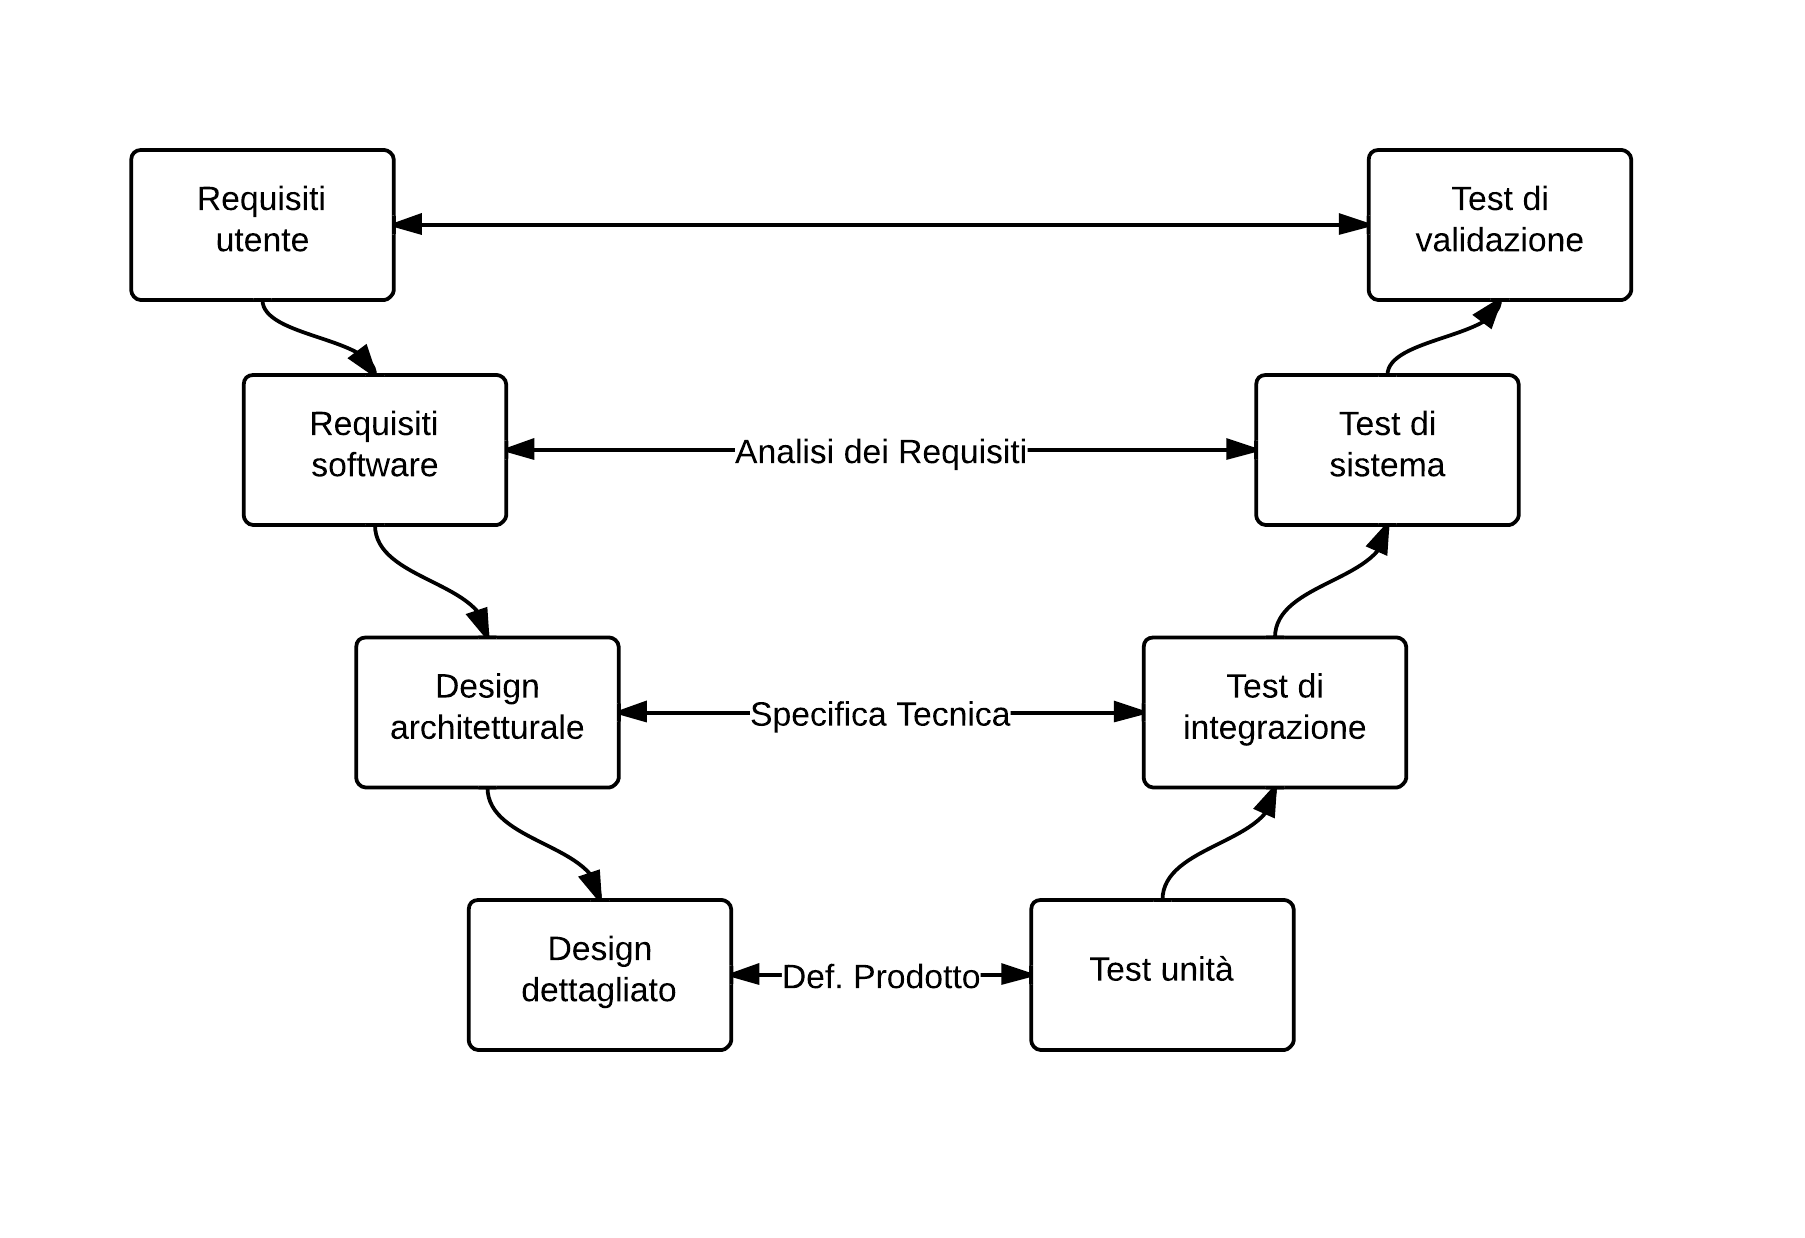
\includegraphics[width=1\textwidth]{V-Model.png}
	\caption{V-Model per il testing software}
	\label{fig:V-Model}
	\end{figure}

	\subsection{Test di sistema}
	Vengono qui descritti i test di sistema che andranno a verificare il funzionamento complessivo delle componenti.
	Nella seguente tabella, lo stato di ogni test è definito da N.E per non eseguito. I requisiti che non sono stati accettati nel \AnalisiDeiRequisiti{} sono qui marcati con un \texttt{*} ad indicare che il test associato non verrà effettuato.
	
	

	\begin{center}
	\def\arraystretch{1.5}
	\bgroup
		\begin{longtable}{| p{3cm} | p{6cm} | p{1.5cm} | p{2cm} | }
		\hline 
		 \textbf{Test Sistema} & \textbf{Descrizione} & \textbf{Stato} & \textbf{Requisito} \\ \hline
				TS-RA1O 1.1 & 
				Verificare che durante la verifica delle credenziali l'indirizzo email venga immesso tramite un campo di testo apposito. & N.E & RA1O 1.1 \newline  \\ \hline 
				TS-RA1O 1.2 & 
				Verificare che durante la verifica delle credenziali, la password venga immessa tramite un capo di testo apposito.
 & N.E & RA1O 1.2 \newline  \\ \hline 
				TS-RA1O 1.3 & 
				Verificare che il sistema verifichi le credenziali di un utente tramite un database indipendente da quello che contiene la Collection. & N.E & RA1O 1.3 \newline  \\ \hline 
				TS-RA1O 1.3.1 & 
				Verificare che, in caso di fallimento dell'autenticazione di un utente, il sistema visualizzi una pagina di errore. & N.E & RA1O 1.3.1 \newline  \\ \hline 
				TS-RA1O 1.3.2 & 
				Verificare che in caso in cui autenticazione vada a buon fine, l'utente venga reindirizzato automaticamente sulla dashboard dell'applicazione.  & N.E & RA1O 1.3.2 \newline  \\ \hline 
				TS-RA1O 2.1 & 
				Verificare che il sistema permetta il recupero password attraverso l'inserimento dell'email.
 & N.E & RA1O 2.1 \newline  \\ \hline 
				TS-RA1O 2.2 & 
				Verificare che un utente non autenticato che richiede il reset della propria password riceva un email con un link per il reset. & N.E & RA1O 2.2 \newline  \\ \hline 
				TS-RA1O 2.3 & 
				Verificare che un utente non autenticato possa resettare la propria password tramite l'inserimento di una nuova password.
 & N.E & RA1O 2.3 \newline  \\ \hline 
				TS-RA1O 4.1 & 
				Verificare che la visualizzazione di una Collection-index consista in una tabella le cui righe corrispondono ai document presenti nel database e le cui colonne siano i relativi attributi. & N.E & RA1O 4.1 \newline  \\ \hline 
				TS-RA1O 4.1.1 & 
				Verificare che ogni riga della tabella corrispondente ad un Document abbia una chiave selezionabile che rimanda alla corrispondente pagina show.
 & N.E & RA1O 4.1.1 \newline  \\ \hline 
				TS-RA1D 4.1.2 & 
				Verificare che l'admin possa eliminare un documento tramite un link rapido. & N.E & RA1D 4.1.2 \newline  \\ \hline 
				TS-RA1D 4.1.3 & 
				Verificare che l'admin possa modificare un document della collection-index.
 & N.E & RA1D 4.1.3 \newline  \\ \hline 
				TS-RA1D 4.2 & 
				Verificare che sia possibile visualizzare un sottoinsieme di Document tramite dei filtri personalizzati sugli attributi. & N.E & RA1D 4.2*  \newline  \\ \hline 
				TS-RA1F 4.3 & 
				Verificare che l'amministratore possa creare un nuovo Document nella base di dati. & N.E & RA1F 4.3*  \newline  \\ \hline 
				TS-RA1O 5.1 & 
				Verificare che l'admin possa editare ogni singolo attributo modificabile del documento della pagina show. & N.E & RA1O 5.1 \newline  \\ \hline 
				TS-RA1F 5.2 & 
				Verificare che l'utente possa eseguire un'azione personalizzata tramite l'esecuzione di un pulsante. & N.E & RA1F 5.2*  \newline  \\ \hline 
				TS-RA1O 5.3 & 
				Viene verificato che l'utente possa eliminare il Document selezionato nella show-page. & N.E & RA1O 5.3 \newline  \\ \hline 
				TS-RA1O 6.1 & 
				Viene verificato che l'admin possa creare un nuovo utente dalla pagina di amministrazione. & N.E & RA1O 6.1 \newline  \\ \hline 
				TS-RA1O 6.1.1 & 
				Viene verificato che l'admin disponga di una pagina di creazione di un nuovo utente. & N.E & RA1O 6.1.1 \newline  \\ \hline 
				TS-RA1O 6.1.1.1 & 
				Verificare che l'admin possa inserire l'indirizzo email del nuovo utente in un apposito campo di testo presente all'interno della pagina di creazione di un nuovo utente. & N.E & RA1O 6.1.1.1 \newline  \\ \hline 
				TS-RA1O 6.1.1.2 & 
				Viene verificato che l'admin possa inserire la password del nuovo utente in un apposito campo di testo presente all'interno della pagina di creazione di un nuovo utente. & N.E & RA1O 6.1.1.2 \newline  \\ \hline 
				TS-RA1O 6.1.1.3 & 
				Verificare che l'admin possa inserire il ``livello utente'' del nuovo utente tramite una combo-box presente all'interno della pagina di creazione di un nuovo utente. & N.E & RA1O 6.1.1.3 \newline  \\ \hline 
				TS-RA1O 6.1.2 & 
				Viene verificato che l'applicazione prelevi tutti i dati inseriti dall'admin nella pagina di creazione di un nuovo utente e li invii al database delle credenziali, il quale provvederà all'inserimento del nuovo record. & N.E & RA1O 6.1.2 \newline  \\ \hline 
				TS-RA1O 6.1.3 & 
				Verificare che venga visualizzato un messaggio d'errore nel caso in cui l'admin non abbia compilato correttamente i campi presenti all'interno della pagina di creazione di un nuovo utente. & N.E & RA1O 6.1.3 \newline  \\ \hline 
				TS-RA1O 6.2 & 
				Viene verificato che l'admin abbia la possibilità di selezionare un utente dalla index-page e visualizzare la sua relativa show-page. & N.E & RA1O 6.2 \newline  \\ \hline 
				TS-RA1O 6.2.1 & 
				Verificare che l'admin possa elevare l'utente normale selezionato al livello ``admin'' dalla show-page relativa. & N.E & RA1O 6.2.1 \newline  \\ \hline 
				TS-RA1O 6.2.2 & 
				Verificare che l'admin possa declassare l'admin selezionato a livello di utente normale dalla show-page relativa. & N.E & RA1O 6.2.2 \newline  \\ \hline 
				TS-RA1O 6.2.3 & 
				Viene verificato che l'admin possa modificare l'attributo email dell'utente selezionato dalla relativa show-page. & N.E & RA1O 6.2.3 \newline  \\ \hline 
				TS-RA1O 6.2.4 & 
				Verificare che l'admin possa modificare l'attributo password dell'utente selezionato dalla relativa show-page. & N.E & RA1O 6.2.4 \newline  \\ \hline 
				TS-RA1O 6.2.5 & 
				Viene verificato che l'admin possa eliminare l'utente visualizzato nella \glossario{show-page}. & N.E & RA1O 6.2.5 \newline  \\ \hline 
				TS-RF1O 7 & 
				Verificare che il linguaggio DSL all'interno di MaaP Framework sia stato implementato e sia funzionante. & N.E & RF1O 7 \newline  \\ \hline 
				TS-RF1O 8.1  & 
				Verificare che Maap Framework generi automaticamente lo scheletro dell’applicazione creata dallo sviluppatore. & N.E & RF1O 8.1  \newline  \\ \hline 
				TS-RF1O 8.1.1 & 
				Verificare che Maap Framework importi automaticamente in un'apposita directory del progetto tutte le librerie necessarie al corretto funzionamento del sistema. Librerie necessarie: \begin{itemize} \item Express v-3.4.8 \item MongoDB v-1.3.23 \item Mongoose v-3.8.4 \end{itemize} & N.E & RF1O 8.1.1 \newline  \\ \hline 
				TS-RF1O 8.1.2 & 
				Verificare che Maap Framework crei automaticamente in un’apposita directory il file di configurazione di default dell’applicazione generata. & N.E & RF1O 8.1.2 \newline  \\ \hline 
				TS-RF1O 8.1.3 & 
				Viene verificato che Maap Framework crei automaticamente il sistema di autenticazione per l’applicazione generata. & N.E & RF1O 8.1.3 \newline  \\ \hline 
				TS-RF1O 8.1.4 & 
				Verificare che Maap Framework crei automaticamente le directory di descrizione delle pagine web. & N.E & RF1O 8.1.4 \newline  \\ \hline 
				TS-RF1O 8.2 & 
				Verificare che Maap Framework crei automaticamente un account admin di default. & N.E & RF1O 8.2 \newline  \\ \hline 
				TS-RF1F 8.3 & 
				Verificare che il framework MaaP permetta allo sviluppatore di definire un namespace per l’applicazione generata. & N.E & RF1F 8.3*  \newline  \\ \hline 
				TS-RF1O 9.1 & 
				Verificare che il DSL permetta allo sviluppatore di creare una pagina Collection-index. & N.E & RF1O 9.1 \newline  \\ \hline 
				TS-RF1O 9.1.1 & 
				Verificare che il DSL deve permetta allo sviluppatore di poter definire una serie di attributi da visualizzare all’interno della pagina Collection-index. & N.E & RF1O 9.1.1 \newline  \\ \hline 
				TS-RF1O 9.1.2 & 
				Viene verificato che il DSL permetta allo sviluppatore di poter definire un ordinamento di default (ordine alfanumerico) di visualizzazione dei document all'interno della pagina Collection-index. & N.E & RF1O 9.1.2 \newline  \\ \hline 
				TS-RF1O 9.1.3 & 
				Verificare che il DSL permetta allo sviluppatore di poter definire un eventuale limite di elementi da visualizzare all’interno della pagina Collection-index. & N.E & RF1O 9.1.3 \newline  \\ \hline 
				TS-RF1O 9.1.4 & 
				Viene verificato che il DSL permetta allo sviluppatore di poter definire quali attributi sono ordinabili all’interno della pagina Collection-index. & N.E & RF1O 9.1.4 \newline  \\ \hline 
				TS-RF1O 9.1.5 & 
				Verificare che il DSL permetta allo sviluppatore di definire la funzione populate per far si che una chiave riferisca ad un documento esterno. & N.E & RF1O 9.1.5 \newline  \\ \hline 
				TS-RF1O 9.1.6 & 
				Verificare che il DSL permetta allo sviluppatore di definire delle query per creare la pagina Collection-index in base al risultato della loro estrazione. & N.E & RF1O 9.1.6 \newline  \\ \hline 
				TS-RF1O 9.1.7 & 
				Viene verificato che il DSL permetta allo sviluppatore di definire delle trasformazioni sugli attributi da visualizzare. & N.E & RF1O 9.1.7 \newline  \\ \hline 
				TS-RF1O 9.2 & 
				Viene verificato che il DSL permetta allo sviluppatore di creare una pagina Collection-show. & N.E & RF1O 9.2 \newline  \\ \hline 
				TS-RF1O 9.2.1 & 
				Verificare che il DSL permetta allo sviluppatore di definire una serie di attributi visualizzabili all’interno della pagina Collection-show. & N.E & RF1O 9.2.1 \newline  \\ \hline 
				TS-RF1O 9.2.2 & 
				Verificare che il DSL permetta allo sviluppatore la definizione degli attributi del Document come attributi innestati o array di Document tramite la funzione populate. & N.E & RF1O 9.2.2 \newline  \\ \hline 
				TS-RF1O 9.2.3 & 
				Verificare che lo sviluppatore abbia la possibilità di personalizzare la show page definendone l’ordinamento degli attributi. & N.E & RF1O 9.2.3 \newline  \\ \hline 
				TS-RF1O 9.2.4 & 
				Viene verificato che lo sviluppatore possa definire trasformazioni agli attributi per poi visualizzarli nella show-page. & N.E & RF1O 9.2.4 \newline  \\ \hline 
				TS-RF1F 9.2.5 & 
				Verificare che lo sviluppatore possa personalizzare la show-page definendo delle operazioni personalizzate che l’utente potrà utilizzare tramite appositi pulsanti. & N.E & RF1F 9.2.5*  \newline  \\ \hline 
				TS-RF1O 9.3 & 
				Viene verificato che il framework MaaP permetta allo sviluppatore di cambiare il nome della Collection da visualizzare nel menu di navigazione. & N.E & RF1O 9.3 \newline  \\ \hline 
				TS-RF1O 9.4 & 
				Verificare che il framework MaaP permetta allo sviluppatore di modificare l’ordine di visualizzazione della Collection nel menu di navigazione. & N.E & RF1O 9.4 \newline  \\ \hline 
				TS-RS1F 10.1 & 
				Verificare che il sistema MaaS permetta allo sviluppatore di scrivere una Collection tramite editor di testo presente nella pagina web. & N.E & RS1F 10.1*  \newline  \\ \hline 
				TS-RS1F 10.2 & 
				Verificare che il sistema MaaS permetta all'utente di poter scrivere una Collection caricando un file prodotto dal framework MaaP. & N.E & RS1F 10.2*  \newline  \\ \hline 
				TS-RS1F 10.3 & 
				Verificare che il sistema MaaS permetta ad un utente non registrato di registrarsi al suo servizio. & N.E & RS1F 10.3*  \newline  \\ \hline 
				TS-RS1F 10.4 & 
				Verificare che il sistema MaaS assegni automaticamente un \glossario{namespace} sul sistema al nuovo utente registrato. & N.E & RS1F 10.4*  \newline  \\ \hline 
				TS-RS1F 10.5 & 
				Verificare che il servizio MaaS visualizzi un messaggio d’errore nel caso in cui la registrazione fallisca a causa di credenziali già esistenti. & N.E & RS1F 10.5*  \newline  \\ \hline 
				TS-RS1F 10.6 & 
				Verificare che il servizio MaaS metta a disposizione di un utente non autenticato la possibilità di effettuare il login al sistema. & N.E & RS1F 10.6*  \newline  \\ \hline 
				TS-RS1F 10.7 & 
				Verificare che il servizio MaaS visualizzi un messaggio d’errore nel caso in cui l’utente non autenticato abbia inserito credenziali errate nel sistema di login. & N.E & RS1F 10.7*  \newline  \\ \hline 
				TS-RS1F 10.8 & 
				Verificare che il sistema MaaS permetta ad un utente non autenticato di modificare il proprio profilo. & N.E & RS1F 10.8*  \newline  \\ \hline 
				TS-RS1F 10.9 & 
				Verificare che il sistema MaaS permetta ad un utente non autenticato di eliminare il proprio account dal sistema. & N.E & RS1F 10.9*  \newline  \\ \hline 
				TS-RS1F 10.9.1 & 
				Verificare che il sistema MaaS provveda all'eliminazione dei file di configurazione associati all'utente rimosso dal sistema. & N.E & RS1F 10.9.1*  \newline  \\ \hline 
				TS-RS1F 10.10 & 
				Verificare che il sistema MaaS permetta allo sviluppatore di eliminare una Collection esistente. & N.E & RS1F 10.10*  \newline  \\ \hline 
				TS-RA1D 13.1 & 
				Verificare che l’utente possa modificare la password di accesso all'applicazione. & N.E & RA1D 13.1 \newline  \\ \hline 
				TS-RF1O 14.1 & 
				Verificare che il framework MaaP renda possibile la configurazione dei database delle credenziali. & N.E & RF1O 14.1 \newline  \\ \hline 
				TS-RF1O 14.2 & 
				Verificare che il framework MaaP renda possibile la configurazione dei database delle Collection. & N.E & RF1O 14.2 \newline  \\ \hline 
				TS-RF1F 14.3 & 
				Verificare che il framework MaaP renda possibile la selezione di un name-space per un database se la funzione di \glossario{namespace} è abilitata. & N.E & RF1F 14.3*  \newline  \\ \hline 
				TS-RA1F 15.1 & 
				Verificare che l’applicazione MaaP metta a disposizione dell’admin la visualizzazione degli indici in base alle query più richieste dall’applicazione. & N.E & RA1F 15.1*  \newline  \\ \hline 
				TS-RA1F 15.2 & 
				Verificare che l’applicazione MaaP permetta all’admin di aggiungere gli indici in base ai suggerimenti forniti. & N.E & RA1F 15.2*  \newline  \\ \hline 
				TS-RA1F 15.3 & 
				Verificare che l’applicazione MaaP permetta all’admin di rimuovere gli indici in base ai suggerimenti forniti. & N.E & RA1F 15.3*  \newline  \\ \hline 
				TS-RS1F 17 & 
				Verificare che Il sistema MaaS si accerti che documenti creati rispettano i vincoli del database. & N.E & RS1F 17*  \newline  \\ \hline 
				TS-RA1O 18 & 
				Verificare che il sistema metta a disposizione un validatore del codice DSL e visualizzi gli eventuali errori logici o di sintassi in un'apposita pagina. & N.E & RA1O 18 \newline  \\ \hline 
				TS-RS1F 19 & 
				Verificare che il sistema MaaS salvi le pagine definite dagli utenti nel database e non su disco. & N.E & RS1F 19*  \newline  \\ \hline 
		\caption{Tracciamento Test di Sistema - Requisiti}
		\end{longtable}
	 \egroup
\end{center}
	
	\subsection{Test di integrazione}
	I test di integrazione vanno a controllare il corretto funzionamento delle componenti descritti dalla progettazione ad alto livello. Si è scelto di utilizzare un approccio \glossario{top-down} ad eccezione del test TI 9 che viene eseguito con la metodologia \glossario{bottom-up}. Di seguito viene riportato un diagramma informale per chiarire l'albero dei test di integrazione.

	\begin{figure}[H]
	\centering 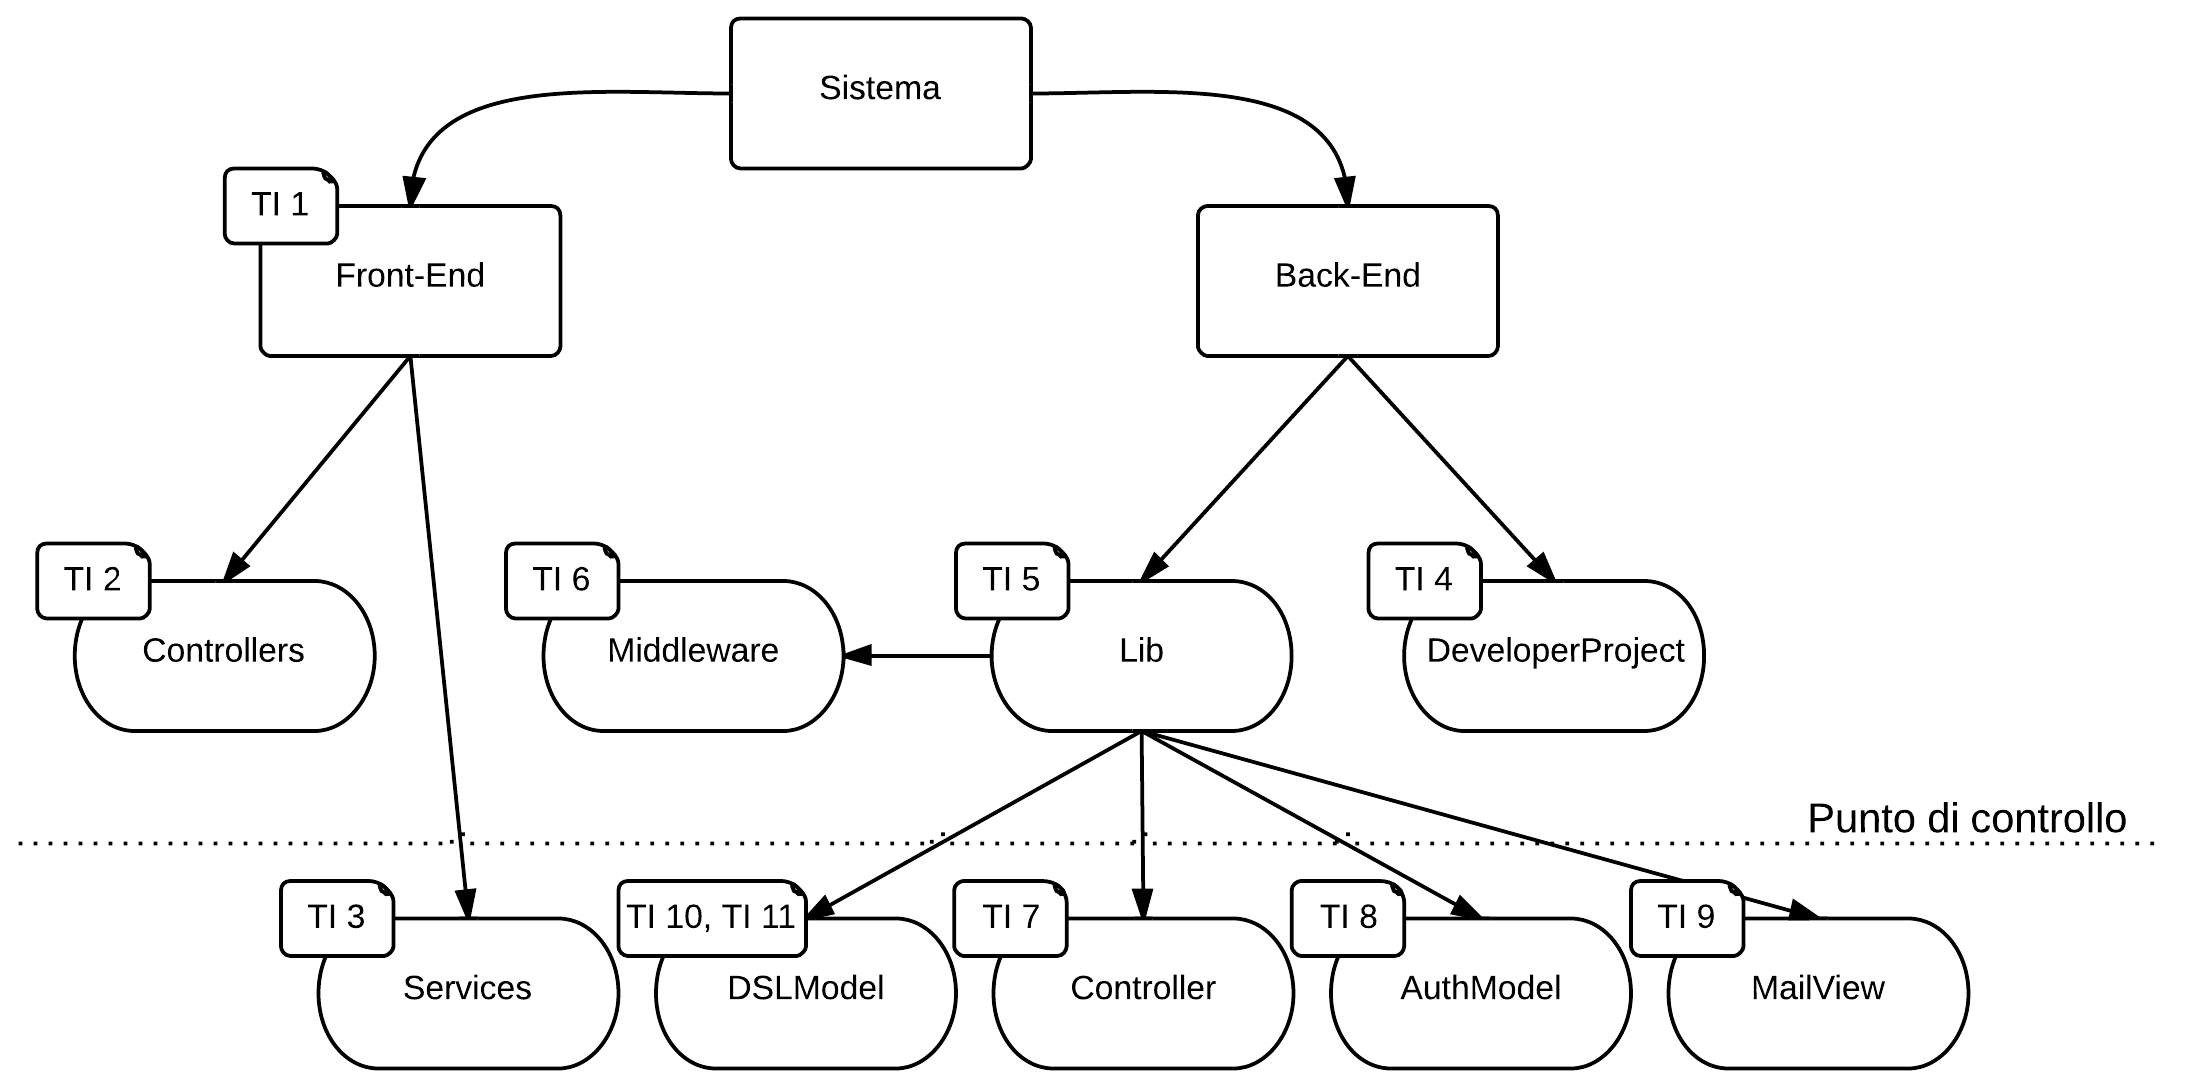
\includegraphics[width=1\textwidth]{sequenza-di-integrazione.png}
	\caption{Sequenza d'integrazione delle componenti}
	\label{fig:sequenza-di-integrazione}
	\end{figure}

	Con la tecnica \glossario{top-down} le componenti di più alto livello sono testate non appena sono implementate. Le componenti del sottosistema che non sono ancora state sviluppate, vengono simulate dagli \glossario{stub}. Man mano che si procede con la codifica delle componenti di più basso livello, queste vengono integrate e viene eseguito il relativo test. Grazie all'integrazione incrementale delle componenti del sistema, è più semplice determinare quale componente crea problemi e le funzioni di più alto livello sono testate prima.

	La componente Front-end::Model non ha associato test d'integrazione poiché le classi di questo \glossario{package} si prevede che non verranno codificate in quanto verrà sfruttato lo stile di \glossario{duck-typing} della gestione dei tipi di \glossario{JavaScript}.

	\begin{figure}[H]
	\centering 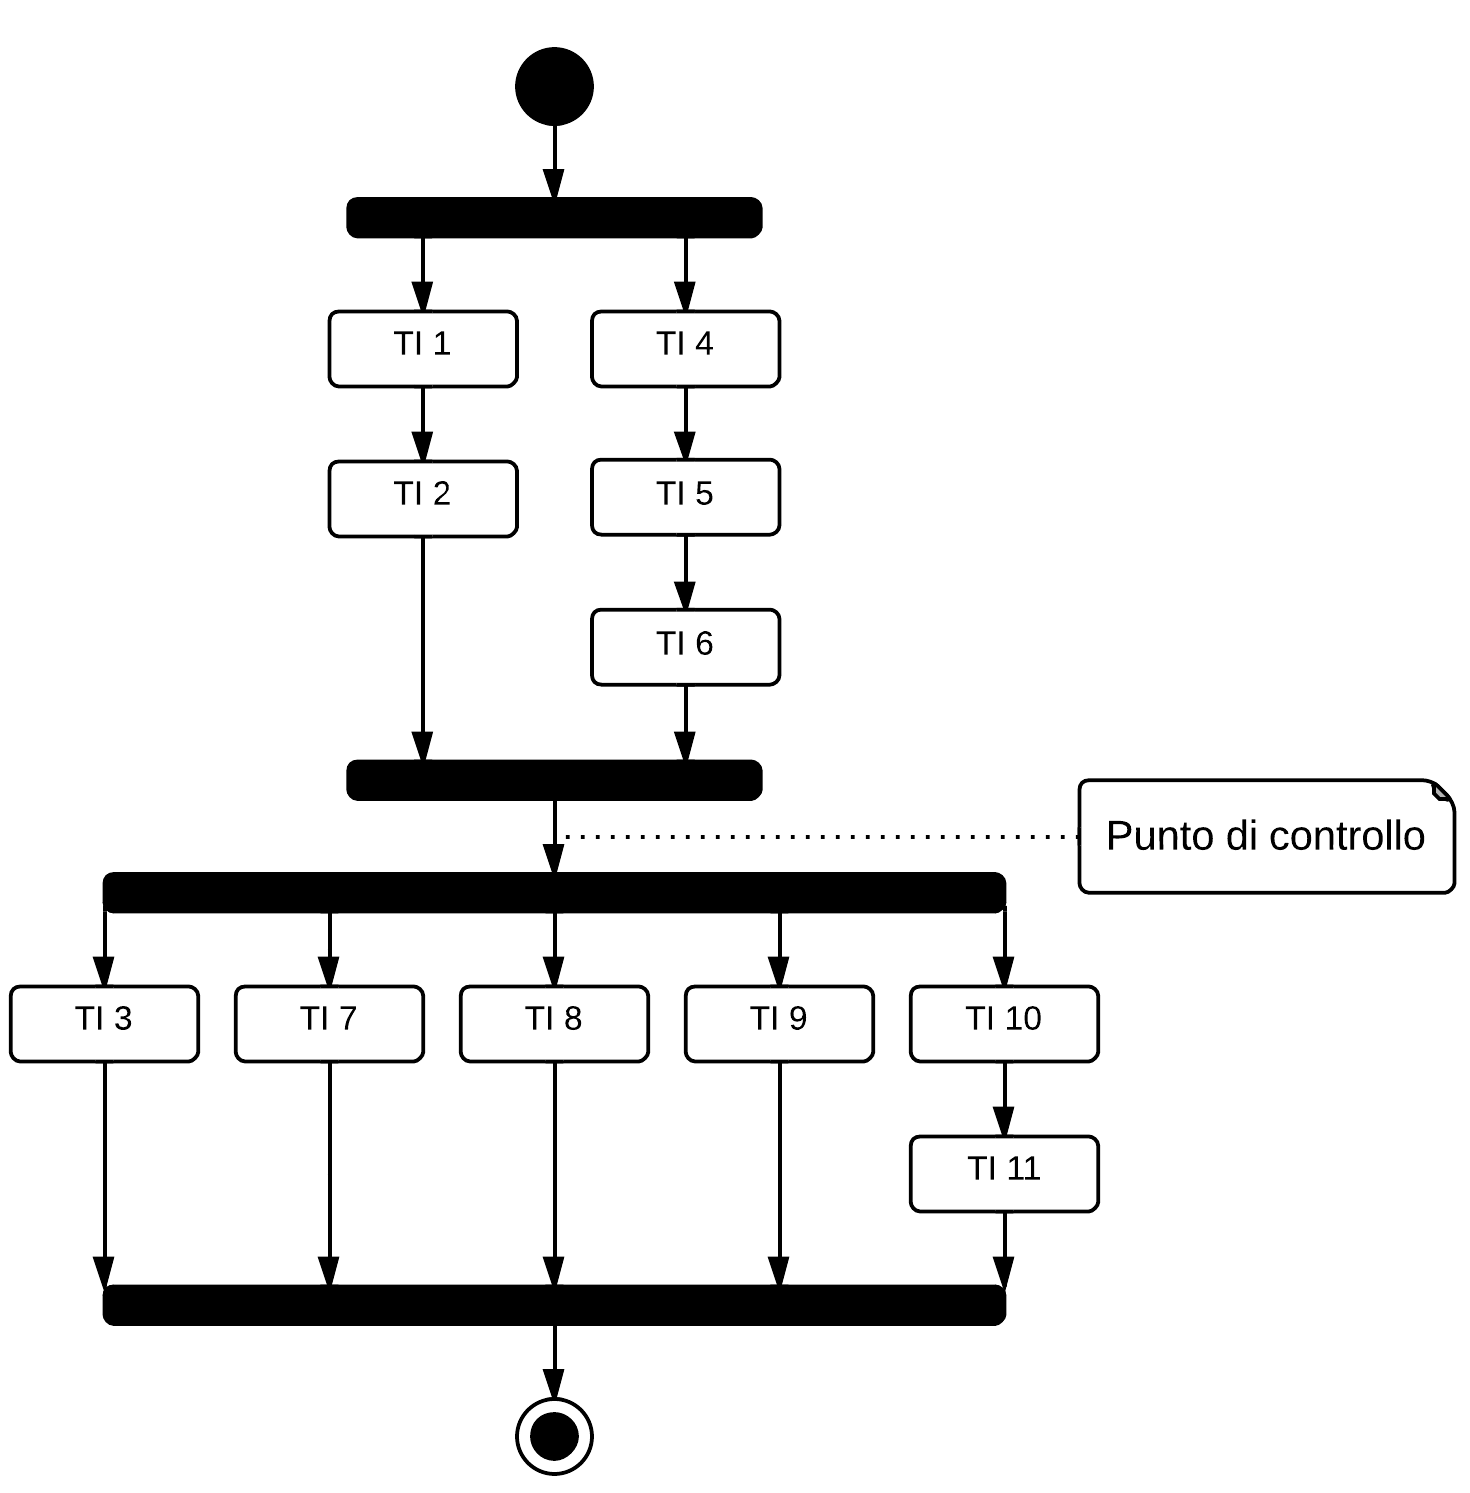
\includegraphics[width=0.59\textwidth]{sequenza-dei-test.png}
	\caption{Diagramma di attività dei test}
	\label{fig:sequenza-dei-test}
	\end{figure}
	
	%TODO tabella: componente / test
	\bgroup
	\begin{longtable}[H]{|P{1cm}|P{5cm}|P{4.5cm}|P{2cm}|}
		\hline \textbf{Test} & \textbf{Descrizione} & \textbf{Componenti aggiunte} & \textbf{Stato} \\
		
		\hline TI 1 & Si verifica che l'applicazione Web carichi correttamente le librerie JavaScript utilizzate. & Front-end & N.E. \\
		\hline TI 2 & Si verifica che i controller si integrino correttamente nell'applicazione Web. & Front-end::Controllers & N.E. \\
		\hline TI 3 & Si verifica che i services permettono di interagire correttamente con il back-end. & Front-end::Services & N.E. \\
		\hline TI 4 & Si verifica che il DeveloperProject avvii correttamente il server, fornendo in particolare i file statici del front-end. & Back-end::DeveloperProject & N.E. \\
		\hline TI 5 & Si verifica che la libreria si integri correttamente con il \glossario{Node Package Manager} (npm) E che il suo script di installazione produca un DeveloperProject funzionante. & Back-end::Lib & N.E. \\
		\hline TI 6 & Si verifica che i controller si integrino correttamente tra loro e nella gestione delle richieste che arrivano al server. & Back-end::Lib::Controller & N.E. \\
		\hline TI 7 & Si verifica che il Middleware si integri correttamente nella gestione delle richieste che arrivano al server. & Back-end::Lib::Controller::Middleware & N.E. \\
		\hline TI 8 & Si verifica che il Service si integri correttamente nella gestione delle richieste che arrivano al server. & Back-end::Lib::Controller::Service & N.E. \\
		\hline TI 9 & Si verifica che il Model si integri correttamente della gestione dell'inserimento, della modifica, della creazione e dell'eliminazione consistente dei dati. & Back-end::Lib::Model & N.E. \\
		\hline TI 10 & Si verifica che la View si integri correttamente con il Middleware per fornire i template come la gestione dell'invio delle mail. & Back-end::Lib::View & N.E. \\
		\hline TI 11 & Si verifica che Utils si integri correttamente con il funzionamento dell'applicazione. & Back-end::Lib::Utils & N.E. \\
		\hline TI 12 & Si verifica che le classi che compongono il DSLModel interagiscano correttamente tra loro. & Back-end::Lib::DSLModel & N.E. \\
		\hline TI 13 & Si verifica che il DSLModel si integri correttamente con il funzionamento dell'applicazione. & Back-end::Lib::DSLModel & N.E. \\
		\hline

	\caption{Descrizione test d'Integrazione}
	\end{longtable}
	\egroup

	\subsection{Test di validazione}
	In questa sezione vengono elencati i test di validazione per verificare che il prodotto sia conforme alle attese. I test si svolgono seguendo e verificano tutti passi di cui si compongono. I requisiti che non sono stati accettati nel \AnalisiDeiRequisiti{} sono qui marcati con un \texttt{*} ad indicare che il test associato non verrà effettuato.
	
	
  \begin{center}
  \def\arraystretch{1.5}
  \bgroup
    \begin{longtable}{| p{3cm} | p{6cm} | p{1.5cm} | p{2cm} | }
    \hline 
     \textbf{Test di Validazione} & \textbf{Descrizione} & \textbf{Stato} & \textbf{Requisito} \\ \hline
        TV-RA1O 1 & 
        L'utente non autenticato intende accedere all'applicazione, per farlo deve inserire le proprie credenziali composte da una email ed una password.
All'utente è richiesto di:
\begin{itemize}
\item Raggiungere la pagina di autenticazione;
\item Inserire la mail nel campo apposito;
\item Inserire la password;
\item Procedere con l'autenticazione.
\end{itemize}
 & N.E &       
            RA1O 1 \newline  \\ \hline 
        TV-RA1O 2 & 
        L'utente intende recuperare la password d'accesso all'applicazione.
All'utente è richiesto di:
\begin{itemize}
\item Essere autenticato;
\item Raggiungere la pagina per il reset della password;
\item Richiedere il reset;
\item Raggiungere la casella email collegata all'account del sistema;
\item Seguire il link contento nella mail:
\item Compilare il form richiedente la nuova password;
\item Eseguire il Logout e autenticarsi con la nuova password.
\end{itemize} & N.E &       
            RA1O 2 \newline  \\ \hline 
        TV-RA1D 3 & 
        L'utente autenticato può visualizzare la pagina di Dashboard nella quale potrà aver accesso ad esempio alla lista delle collection presenti e ad altre funzionalità disponibili.
All'utente è richiesto di:
\begin{itemize}
\item Accertarsi di essere autenticato;
\item Accedere alla pagina Dashboard tramite il menu di navigazione;
\end{itemize} & N.E &       
            RA1D 3 \newline  \\ \hline 
        TV-RA1O 4 & 
        L'utente autenticato, selezionata una \glossario{Collection}, ne visualizza in forma tabellare tutti i documenti che contiene. \newline Di questa collection può filtrarne i risultati visualizzabili, può eseguire tramite bottoni predisposti nella pagina azioni personalizzati e per ogni \glossario{Document}, selezionarlo e visualizzarne la show-page corrispondente. \newline L'Admin ha i permessi per modificare un documento o eliminare un \glossario{Document}. \newline
All'utente è richiesto di:
\begin{itemize}
\item Essere autenticato;
\item Aprire la show-page relativa ad un Document;
\item Usare i filtri per filtrare la Collection
\item Eseguire un azione personalizzata, laddove presente;
\item Se admin, modificare un Document;
\item Se admin, eliminare un Document;
\end{itemize} & N.E &       
            RA1O 4 \newline  \\ \hline 
        TV-RA1O 5 & 
        L'utente visualizza la pagina show-page corrispondente ad un \glossario{Document} selezionato visualizzandone gli attributi in forma tabellare. \newline In questa pagina può aprire la show-page o l'index-page dell'array di \glossario{Document} degli attributi innestati se presenti, eseguire un'operazione personalizzata se disponibile. \newline L'Admin può eliminare il \glossario{Document} a cui la show-page corrisponde o modificarlo. 
All'utente è richiesto di:
\begin{item}
\item Essere autenticato;
\item Aprire la show-page degli attributi innestati;
\item Aprire l'index-page dell'arra di Document;
\item Eseguire, se presente, un operazione personalizzata;
\item Se admin, modificare il Document;
\item Se admin, eliminare il Document.
\end{item} & N.E &       
            RA1O 5 \newline  \\ \hline 
        TV-RA1O 6 & 
        L'Admin entra nella sua pagina di amministrazione nella quale visualizza una \glossario{Collection-Index} di tutti gli utenti registrati al sistema.
All'utente è richiesto di:
\begin{itemize}
\item Essere autenticato come admin;
\item Accedere alla pagina di creazione nuovi utenti;
\item Creare un nuovo utente;
\item Accedere alla pagina degli utenti registrati al sistema;
\item Visualizzare la pagina Collection-Show di un utente;
\end{itemize}
 & N.E &       
            RA1O 6 \newline  \\ \hline 
        TV-RF1O 8 & 
        Lo sviluppatore deve poter creare un nuovo progetto tramite linea di comando.
\newline
Allo sviluppatore è richiesto di:
\begin{itemize}
\item Richiamare il comando di creazione di un nuovo progetto;
\item Passare come parametro il nome della directory che conterrà il progetto;
\item Verificare che siano state importate le librerie necessarie al corretto funzionamento del sistema;
\item Verificare che sia stato creato il file di configurazione di default dell’applicazione generata;
\item Verificare che sia stato creato il sistema di autenticazione per l’applicazione generata;
\item Verificare che siano state create le directory di descrizione delle pagine web;
\item Verificare che sia stato creato un account admin di default.
\end{itemize} & N.E &       
            RF1O 8 \newline  \\ \hline 
        TV-RF1O 9 & 
        Lo sviluppatore deve poter configurare le Collection tramite il DSL di Maap Framework.
All'utente è richiesto di:
\begin{itemize}
\item creare una Collection-index tramite DSL;
\item creare una Collection-show tramite DSL;
\item modificare il nome della Collection;
\item modificare l'ordine di visualizzazione della Collection.
\end{itemize} & N.E &       
            RF1O 9 \newline  \\ \hline 
        TV-RS1F 10 & 
        L'utente autenticato verifica che il \glossario{framework} MaaP sia messo a disposizione dal sistema \glossario{MaaS} come servizio Web.
\newline
All'utente è richiesto di:
\begin{itemize}
\item Accedere alla pagina di modifica del proprio profilo;
\item Modificare i dati associati al proprio profilo;
\item Verificare che i dati siano stati aggiornati;
\item Gestire i file di configurazione;
\item Eliminare il proprio account;
\item Verificare l'inaccessibilità al servizio tramite l'autenticazione con le credenziali associate all'account eliminato.
\end{itemize} & N.E &       
            RS1F 10 \newline  \\ \hline 
        TV-RA1D 11 & 
        L'utente non autenticato deve potersi registrare all'applicazione MaaP.
\newline
All'utente è richiesto di:
\begin{itemize}
\item Inserire la mail nell'apposito campo di testo;
\item Inserire la password nell'apposito campo di testo;
\item Verificare che l'account sia stato registrato tramite l'autenticazione all'applicazione.
\end{itemize} & N.E &       
            RA1D 11 \newline  \\ \hline 
        TV-RA1D 12 & 
        L'utente autenticato deve poter eseguire il logout dall'applicazione.
\newline
All'utente è richiesto di:
\begin{itemize}
\item Selezionare l'apposita opzione di logout;
\item Verificare di non essere più autenticato.
\end{itemize} & N.E &       
            RA1D 12 \newline  \\ \hline 
        TV-RA1D 13 & 
        L'utente autenticato deve poter modificare le proprie credenziali d'accesso all'interno della propria pagina profilo.
\newline
All'utente viene richiesto di:
\begin{itemize}
\item Accedere alla propria pagina profilo;
\item Modificare la propria mail;
\item Modificare la propria password;
\item Eseguire il logout;
\item Autenticarsi con le nuove credenziali.
\end{itemize} & N.E &       
            RA1D 13 \newline  \\ \hline 
        TV-RF1O 14 & 
        Lo sviluppatore deve poter configurare i database che compongono il sistema MaaP.
\newline
Allo sviluppatore è richiesto di:
\begin{itemize}
\item Configurare la connessione al database delle credenziali degli utenti;
\item Configurare il \glossario{namespace} corrispondente, se la funzione di \glossario{namespace} è abilitata;
\item Configurare la connessione al database delle \glossario{Collection};
\item Configurare il \glossario{namespace} corrispondente, se la funzione di \glossario{namespace} è abilitata;
\item Selezionare un \glossario{namespace} per il database da configurare, se la funzione di \glossario{namespace} è abilitata.
\end{itemize} & N.E &       
            RF1O 14 \newline  \\ \hline 
        TV-RA1F 15 & 
        L'admin deve poter gestire gli indici da un'apposita pagina.
\newline
All'admin è richiesto di:
\begin{itemize}
\item Accedere alla pagina di gestione degli indici;
\item Visualizzare i suggerimenti per la creazione degli indici;
\item Creare un indice;
\item Creare un indice da quelli suggeriti;
\item Eliminare un indice;
\item Eliminare un indice da quelli suggeriti.
\end{itemize} & N.E &       
            RA1F 15 \newline  \\ \hline 
        TV-RF1F 16 & 
        Lo sviluppatore deve poter abilitare i \glossario{namespace} per l’applicazione creata.
\newline
Allo sviluppatore è richiesto di:
\begin{itemize}
\item Attivare il \glossario{namespace}.
\end{itemize} & N.E &       
            RF1F 16 \newline  \\ \hline 
    \caption{Tracciamento Test di Validazione - Requisiti}
    \end{longtable}
   \egroup
\end{center}
	
	
	\subsection{Test di unità}
	
	\begin{center}
\bgroup
\def\arraystretch{1.5}
\begin{longtable}{ | p{3cm} | p{9cm} | p{2cm} | }
\hline
\cellcolor[gray]{0.9} \textbf{Nome} & \cellcolor[gray]{0.9} \textbf{Descrizione} & \cellcolor[gray]{0.9} \textbf{Stato}
 \\ \hline
TU - 2 & Verifica che il service sia stato iniettato correttamente. & Success \\ \hline
TU - 4 & Il costruttore ServerLoader viene invocato con alcuni oggetti di configurazione di tipo Config predefiniti. Si verifica che in ogni caso l'oggetto ServerLoader costruito sia effettivamente configurato con i parametri forniti in input. & Success \\ \hline
TU - 5 & Viene verificato che un oggetto della classe, dati determinati input, venga costruito in modo corretto secondo quanto atteso. & Success \\ \hline
TU - 6 & Viene verificato che il metodo restituisca l'errore in formato JSON atteso. & Success \\ \hline
TU - 7 & Viene verificato che il metodo restituisca l'errore in formato stringa atteso. & Success \\ \hline
TU - 8 & Viene verificato che il metodo restituisca l'errore in formato \texttt{Error} di \glossario{Node.js} atteso. & Success \\ \hline
TU - 9 & Verifica, iniettando un service, che lo scope venga popolato correttamente. & Success \\ \hline
TU - 10 & Viene simulato uno scope tramite rootScope.new() e un service per testare che il controller gestisca correttamente l'invocazione dei metodi sul service per la modifica dell'utente e il popolamento dello scope. & Success \\ \hline
TU - 11 & Verifica, iniettando un service, che il login venga effettuato quando i dati inseriti sono corretti e visualizzi correttamente l'errore altrimenti. & Success \\ \hline
TU - 12 & Viene verificato che un oggetto della classe venga costruito correttamente secondo quanto atteso. & Success \\ \hline
TU - 13 & Viene verificato che il metodo, dati determinati input, effettui una chiamata alla classe Back-end::Lib::Model::DSLModel::DSLConcreteStrategy e che quest'ultima restituisca tramite una callback un array di collections da inserire nel registro. Viene inoltre verificato che nel caso in cui venga passato in input il nome di un file non esistente il metodo generi un opportuno errore da restituire con una callback. & Success \\ \hline
TU - 14 & Viene verificato che il metodo, dati determinati input, aggiunga correttamente il CollectionModel passatogli al registro dei modelli. & Success \\ \hline
TU - 15 & Viene verificato che il metodo, dato l'id della collection, ne restituisca il model. & Success \\ \hline
TU - 16 & Viene verificato che il metodo restituisca l'array di errori atteso. & Success \\ \hline
TU - 17 & Viene verificato che il metodo inizializzi correttamente lo Schema mongoose degli utenti e renda disponibili i metodi attesi su di esso. & Success \\ \hline
TU - 18 & Viene verificato che il metodo restituisca i dati degli utenti nel formato JSON atteso e gestisca gli eventuali errori di connessione a MongoDB. & Success \\ \hline
TU - 19 & Viene verificato che il metodo, dato il suo input, registri correttamente l'utente nel database e gestisca nel modo atteso gli eventuali errori. & Success \\ \hline
TU - 20 & Viene verificato che il metodo, dato il suo input, modifichi correttamente il livello dell'utente indicato e gestisca nel modo atteso gli eventuali errori. & Success \\ \hline
TU - 21 & Viene verificato che il metodo, dati i suoi input, crei correttamente l'utente atteso sul database MongoDB degli utenti e gestisca gli eventuali errori generati. & Success \\ \hline
TU - 23 & Viene verificato che il metodo, dati i suoi input, modifichi correttamente la password dell'utente indicato la nuova fornita e gestisca gli eventuali errori generati nella maniera attesa. & Success \\ \hline
TU - 24 & Viene verificato che il metodo, dato un id, ricerchi l'utente indicato all'interno del database MongoDB degli utenti restituendo le informazioni associate e gestisca gli eventuali errori generati. & Success \\ \hline
TU - 25 & Viene verificato che il metodo costruisca un oggetto della classe nel modo corretto e atteso. & Success \\ \hline
TU - 26 & Viene verificato che il metodo inizializzi correttamente la classe e gestisca nel modo atteso gli eventuali errori generati. & Success \\ \hline
TU - 27 & Viene verificato che il metodo, dati determinati input, carichi correttamente il file DSL, lo esegua in modo corretto e gestisca in modo atteso gli eventuali errori generati. & Success \\ \hline
TU - 28 & Viene verificato che un oggetto della classe, dati determinati input, venga costruito correttamente e secondo le attese. Viene verificato inoltre che il metodo gestisca correttamente gli eventuali errori generati. & Success \\ \hline
TU - 29 & Viene verificato che il metodo restituisca correttamente il nome della Collection dell'oggetto su cui viene invocato in formato stringa, secondo quanto atteso. & Success \\ \hline
TU - 30 & Viene verificato che il metodo restituisca secondo quanto atteso l' \texttt{IndexModel} dell'oggetto su cui viene invocato. & Success \\ \hline
TU - 31 & Viene verificato che il metodo restituisca secondo quanto atteso lo \texttt{ShowModel} dell'oggetto su cui viene invocato. & Success \\ \hline
TU - 32 & Viene verificato che il metodo, dato il suo input, setti correttamente e in modo atteso il campo \texttt{indexModel} dell'oggetto su cui viene invocato. & Success \\ \hline
TU - 33 & Viene verificato che il metodo, dato il suo input, setti correttamente e in modo atteso il campo \texttt{showModel} dell'oggetto su cui viene invocato. & Success \\ \hline
TU - 34 & Viene verificato che un oggetto della classe venga costruito correttamente dato un certo input. & Success \\ \hline
TU - 35 & Viene verificato che il metodo, dato il suo input, aggiunga in modo corretto e atteso l'attributo indicato all'array \texttt{attributes} dell'oggetto. & Success \\ \hline
TU - 36 & Viene verificato che il metodo restituisca correttamente l'array \texttt{attributes} dell'oggetto su cui viene invocato e che quest'ultimo sia coerente rispetto a quanto atteso. & Success \\ \hline
TU - 37 & Viene verificato che il metodo, dato il suo input, restituisca correttamente e in maniera coerente rispetto a quanto atteso la configurazione della \textit{index-page} in formato JSON. Viene verificato inoltre che il metodo gestisca in modo corretto e atteso gli eventuali errori generati. & Success \\ \hline
TU - 38 & Viene verificato che un oggetto della classe venga costruito correttamente dato un certo input. & Success \\ \hline
TU - 39 & Viene verificato che il metodo, dato il suo input, aggiunga in modo corretto e atteso l'attributo indicato all'array \texttt{attributes} dell'oggetto. & Success \\ \hline
TU - 40 & Viene verificato che il metodo restituisca correttamente l'array \texttt{attributes} dell'oggetto su cui viene invocato e che quest'ultimo sia coerente rispetto a quanto atteso. & Success \\ \hline
TU - 41 & Viene verificato che il metodo, dato il suo input, restituisca correttamente e in maniera coerente rispetto a quanto atteso la configurazione della \textit{show-page} in formato JSON. Viene verificato inoltre che il metodo gestisca in modo corretto e atteso gli eventuali errori generati. & Success \\ \hline
TU - 42 & Viene verificato che un oggetto della classe venga costruito correttamente a partire da valori presi in input. Il test deve verificare inoltre che il metodo sia in grado di gestire gli eventuali errori generati dall'inserimento di un input scorretto. & Success \\ \hline
TU - 43 & Viene verificato che il metodo restituisca correttamente il campo \texttt{label} dell'oggetto sul quale viene invocato e che quest'ultimo sia una stringa e sia coerente rispetto a quanto atteso. & Success \\ \hline
TU - 44 & Viene verificato che il metodo restituisca correttamente il campo \texttt{name} dell'oggetto sul quale viene invocato e che quest'ultimo sia una stringa e sia coerente rispetto a quanto atteso. & Success \\ \hline
TU - 45 & Viene verificato che il metodo restituisca correttamente il campo \texttt{transformation} dell'oggetto sul quale viene invocato e che quest'ultimo sia una \textit{function} e sia coerente rispetto a quanto atteso. & Success \\ \hline
TU - 46 & Viene verificato che il metodo restituisca correttamente il campo \texttt{selectable} dell'oggetto sul quale viene invocato e che quest'ultimo sia di tipo \textit{Boolean} e sia coerente rispetto a quanto atteso. & Success \\ \hline
TU - 47 & Viene verificato che il metodo restituisca correttamente il campo \texttt{sortable} dell'oggetto sul quale viene invocato e che quest'ultimo sia di tipo \textit{Boolean} e sia coerente rispetto a quanto atteso. & Success \\ \hline
TU - 48 & Viene verificato che il metodo comunichi correttamente con lo \texttt{UserModel} richiedendo l'eliminazione dell'utente ricevuto come parametro nella richiesta del server e che sappia gestire correttamente e in modo atteso gli eventuali errori generati. & Success \\ \hline
TU - 49 & Viene verificato che il metodo comunichi correttamente con lo \texttt{UserModel} richiedendo la registrazione dell'utente ricevuto come parametro nella richiesta del server e che sappia gestire correttamente e in modo atteso gli eventuali errori generati. & Success \\ \hline
TU - 50 & Viene verificato che il metodo comunichi correttamente con lo \texttt{UserModel} richiedendo la creazione dell'utente ricevuto come parametro nella richiesta del server e che sappia gestire correttamente e in modo atteso gli eventuali errori generati. & Success \\ \hline
TU - 51 & Viene verificato che il metodo comunichi correttamente con lo \texttt{UserModel} richiedendo i dati dell'utente ricevuto come parametro nella richiesta del server in formato JSON e che sappia gestire correttamente e in modo atteso gli eventuali errori generati. & Success \\ \hline
TU - 52 & Viene verificato che il metodo comunichi correttamente con lo \texttt{UserModel} richiedendo la lista degli utenti presenti nel database MongoDB degli utenti in formato JSON e che sappia gestire correttamente e in modo atteso gli eventuali errori generati. & Success \\ \hline
TU - 53 & Viene verificato che il metodo comunichi correttamente con lo \texttt{UserModel} richiedendo la modifica del livello dell'utente ricevuto come parametro nella richiesta del server e che sappia gestire correttamente e in modo atteso gli eventuali errori generati. & Success \\ \hline
TU - 54 & Viene verificato che il metodo comunichi correttamente con la classe \texttt{DSLCollectionModel} e che ottenga correttamente la configurazione della \textit{index-page} in formato JSON secondo quanto atteso. Viene verificato inoltre che il metodo sia in grado di gestire correttamente gli eventuali errori generati. & Success \\ \hline
TU - 55 & Viene verificato che venga costruito correttamente l'oggetto, configurando il servizio di invio mail con i parametri impostati nella configurazione dell'applicazione passata come parametro. & Success \\ \hline
TU - 56 & Viene verificato che il metodo restituisca un puntatore alla classe Back-end::Lib::Controller::Controller::CollectionController e che quest'ultimo non sia nullo. & Success \\ \hline
TU - 57 & Viene verificato che il metodo restituisca un puntatore alla classe Back-end::Lib::Controller::Controller::ProfileController e che quest'ultimo non sia nullo. & Success \\ \hline
TU - 58 & Viene verificato che il metodo restituisca un puntatore alla classe Back-end::Lib::Controller::Controller::AuthController e che quest'ultimo non sia nullo. & Success \\ \hline
TU - 59 & Viene verificato che il metodo restituisca un puntatore alla classe Back-end::Lib::Controller::Controller::ForgotController e che quest'ultimo non sia nullo. & Success \\ \hline
TU - 60 & Viene verificato che il metodo restituisca un puntatore alla classe Back-end::Lib::Controller::Controller::UserController e che quest'ultimo non sia nullo. & Success \\ \hline
TU - 61 & Viene verificato che il metodo restituisca un puntatore alla classe Back-end::Lib::Controller::Controller::ShowController e che quest'ultimo non sia nullo. & Success \\ \hline
TU - 62 & Viene verificato che il metodo restituisca un puntatore alla classe Back-end::Lib::Controller::Controller::IndexController e che quest'ultimo non sia nullo. & Success \\ \hline
TU - 63 & Viene verificato che un oggetto della classe venga costruito in modo corretto e secondo le attese. & Success \\ \hline
TU - 64 & Viene verificato che il metodo, dato il suo input, invochi correttamente il metodo \texttt{browseFileSystem} andando a cercare tutti i file DSL e successivamente invochi correttamente il metodo di caricamento dei file DSL, andando a costruire quindi il \texttt{DSLModel}. Viene verificato inoltre che il metodo gestisca correttamente gli eventuali errori generati dalle chiamate alle varie funzioni. & Success \\ \hline
TU - 66 & Viene verificato che il metodo, dato il suo input, restituisca  correttamente e in modo atteso l'array di file presenti ne path indicato tramite una callback e sappia gestire in modo corretto e atteso gli eventuali errori generati. & Success \\ \hline
TU - 67 & Viene verificato che il metodo configuri correttamente la gestione delle uri specificate nella sezione ``Interfaccia REST'' della \SpecificaTecnica{}. Per far questo, verrà passato come parametro app un oggetto fittizio, i cui metodi conterranno il codice necessario a verificare che vengano configurate tutte e sole le uri della specifica, associandole ai giusti controller. & Success \\ \hline
TU - 67 & Viene verificato che il metodo, dato il suo input (che sarà una richiesta del server), si interfacci correttamente con la classe \texttt{ShowModel} e restituisca dunque al server la configurazione della show-page attesa in formato JSON. Viene verificato inoltre che il metodo sappia gestire correttamente gli eventuali errori generati.  & Success \\ \hline
TU - 68 & Viene verificato che il metodo inserisca nell'oggetto di risposta res gli errori nel formato JSON generati dal parametro err, impostando il corretto codice HTTP di errore. & Success \\ \hline
TU - 69 & Viene verificato che il metodo inserisca nell'oggetto di risposta res i dati attesi, cioè l'errore nel formato JSON che segnala al client che la richiesta ricevuta richiede una risorsa che non è stata trovata. Deve anche essere impostando il corretto codice HTTP di errore. & Success \\ \hline
TU - 71 & Viene verificato che il metodo, dato il suo input (che sarà una richiesta dal server), si interfacci correttamente con la class \texttt{ShowModel}, la quale si  occuperà di eliminare il Document indicato. Viene verificato inoltre che il metodo sappia gestire gli eventuali errori generati. & Success \\ \hline
TU - 72 & Viene verificato che il metodo, dato il suo input (che sarà una richiesta del server), reindirizzi correttamente l'utente alla Dashboard dell'applicazione. & Success \\ \hline
TU - 73 & Viene verificato che il metodo, dato il suo input (che sarà una richiesta del server), distrugga correttamente la sessione dell'utente indicato e reindirizzi l'utente alla pagina di login. Viene verificato inoltre che il metodo sappia gestire correttamente gli eventuali errori generati. & Success \\ \hline
TU - 74 & Viene verificato che il metodo, dato il suo input (che sarà una richiesta del server), si interfacci correttamente con la classe \texttt{UserModel} e restituisca dunque correttamente e in modo atteso al server i dati dell'utente richiesto in formato JSON. Viene verificato inoltre che il metodo sappia gestire correttamente gli eventuali errori generati. & Success \\ \hline
TU - 75 & Viene verificato che il metodo, dato il suo input (che sarà una richiesta del server), si interfacci correttamente con la classe \texttt{UserModel} ed effettui correttamente l'update della nuova password dell'utente indicato, secondo quanto atteso. Viene verificato inoltre che il metodo sappia gestire correttamente gli eventuali errori generati. & Success \\ \hline
TU - 76 & Viene verificato che il metodo restituisca correttamente al server un errore 404. & Success \\ \hline
TU - 77 & Viene verificato che il metodo, dato il suo input, generi correttamente e in modo atteso il token di reset password e invii correttamente un'email all'indirizzo indicato. Viene verificato inoltre che il metodo sappia gestire in modo corretto gli eventuali errori generati. & Success \\ \hline
TU - 78 & Viene verificato che il metodo, dato i suoi input, restituisca correttamente e in modo atteso l'array dei file presenti nella root indicata tramite una callback. Viene verificato inoltre che il metodo sappia gestire correttamente gli eventuali errori generati. & Success \\ \hline
TU - 79 & Viene verificato che il metodo verifichi se l'utente autenticato ha un livello admin e che gestisca correttamente e in modo atteso gli eventuali errori generati. & Success \\ \hline
TU - 80 & Viene verificato che il metodo verifichi se l'utente è autenticato e che gestisca correttamente e in modo atteso gli eventuali errori generati. & Success \\ \hline
TU - 81 & Viene verificato che il metodo verifichi se l'utente è autenticato e che gestisca correttamente e in modo atteso gli eventuali errori generati. & Success \\ \hline
TU - 82 & Viene verificato che il metodo verifichi se l'utente ha livello di super admin e che gestisca correttamente e in modo atteso gli eventuali errori generati. & Success \\ \hline
TU - 82 & Viene simulato un backend tramite httpBackend per testare che il service richieda e riceva in modo corretto la risorsa user. & Success \\ \hline
TU - 83 & Viene simulato un backend tramite httpBackend per testare che il service richieda in modo corretto la modifica di una risorsa user. & Success \\ \hline
TU - 84 & Viene simulato un backend tramite httpBackend per testare che il service richieda in modo corretto la modifica di una risorsa user. & Success \\ \hline
TU - 85 & Viene simulato un backend tramite httpBackend per testare che il service richieda e riceva in modo corretto la risorsa document richiesta. & Success \\ \hline
TU - 86 & Viene simulato un backend tramite httpBackend per testare che il service richieda e riceva in modo corretto le risorse document di una collection. & Success \\ \hline
TU - 87 & Viene simulato un backend tramite httpBackend per testare che il service richieda e riceva in modo corretto le collection presenti. & Success \\ \hline
TU - 88 & Viene simulato un backend tramite httpBackend per testare che il service richieda in modo corretto la creazione di una risorsa user. & Success \\ \hline
TU - 89 & Viene simulato un backend tramite httpBackend per testare che il service richieda in modo corretto l'eliminazione di una risorsa user. & Success \\ \hline
TU - 90 & Viene simulato un backend tramite httpBackend per testare che il service richieda e riceva in modo corretto le risorse user. & Success \\ \hline
TU - 91 & Viene simulato un backend tramite httpBackend per testare che il service richieda in modo corretto la modifica della risorsa user. & Success \\ \hline
TU - 92 & Viene simulato un backend tramite httpBackend per testare che il service richieda e riceva in modo corretto la risorsa user. (Dell'user loggato) & Success \\ \hline
TU - 93 & Viene simulato uno scope tramite rootScope.new() e un service per testare che il controller gestisca correttamente il prelievo dati dallo scope e l'invocazione dei metodi sul service. & Success \\ \hline
TU - 94 & Si verifica che il controller popoli correttamente i campi dello scope.Lo scope e i service vengono forniti al metodo come stub, in particolare lo scope viene utilizzato per fornire l'output e i service per dare l'input al metodo. Questo test verrà eseguito per tanti valori predefiniti d input e output. & Success \\ \hline
TU - 95 & Si verifica che il controller popoli correttamente i campi dello scope.Lo scope e i service vengono forniti al metodo come stub, in particolare lo scope viene utilizzato per fornire l'output e i service per dare l'input al metodo. Questo test verrà eseguito per tanti valori predefiniti d input e output. & Success \\ \hline
TU - 96 & Viene simulato uno scope tramite rootScope.new() e un service per testare che il controller gestisca correttamente l'invocazione dei metodi sul service per la cancellazione e l'aggiornamento dello scope. & Success \\ \hline
TU - 97 & Si verifica che il controller popoli correttamente i campi dello scope.Lo scope e i service vengono forniti al metodo come stub, in particolare lo scope viene utilizzato per fornire l'output e i service per dare l'input al metodo. Questo test verrà eseguito per tanti valori predefiniti d input e output. & Success \\ \hline
TU - 98 & Si verifica che il controller popoli correttamente i campi dello scope.Lo scope e i service vengono forniti al metodo come stub, in particolare lo scope viene utilizzato per fornire l'output e i service per dare l'input al metodo. Questo test verrà eseguito per tanti valori predefiniti d input e output.
 & Success \\ \hline
TU - 99 & Si verifica che il controller popoli correttamente i campi dello scope.Lo scope e i service vengono forniti al metodo come stub, in particolare lo scope viene utilizzato per fornire l'output e i service per dare l'input al metodo. Questo test verrà eseguito per tanti valori predefiniti d input e output. & Success \\ \hline
TU - 100 & Si verifica che il controller popoli correttamente i campi dello scope.Lo scope e i service vengono forniti al metodo come stub, in particolare lo scope viene utilizzato per fornire l'output e i service per dare l'input al metodo. Questo test verrà eseguito per tanti valori predefiniti d input e output. & Success \\ \hline
TU - 101 & Si verifica che il controller popoli correttamente i campi dello scope.Lo scope e i service vengono forniti al metodo come stub, in particolare lo scope viene utilizzato per fornire l'output e i service per dare l'input al metodo. Questo test verrà eseguito per tanti valori predefiniti d input e output. & Success \\ \hline
TU - 102 & Viene simulato uno scope tramite rootScope.new() e un service per testare che il controller venga costruito correttamente.
 & Success \\ \hline
TU - 103 & Si verifica che il controller popoli correttamente i campi dello scope.Lo scope e i service vengono forniti al metodo come stub, in particolare lo scope viene utilizzato per fornire l'output e i service per dare l'input al metodo. Questo test verrà eseguito per tanti valori predefiniti d input e output.
 & Success \\ \hline
TU - 104 & Si verifica che il controller venga costruito correttamente. & Success \\ \hline
TU - 105 & Si verifica che il controller popoli correttamente i campi dello scope.Lo scope e i service vengono forniti al metodo come stub, in particolare lo scope viene utilizzato per fornire l'output e i service per dare l'input al metodo. Questo test verrà eseguito per tanti valori predefiniti d input e output.
 & Success \\ \hline
TU - 106 & Si verifica che il controller popoli correttamente i campi dello scope.Lo scope e i service vengono forniti al metodo come stub, in particolare lo scope viene utilizzato per fornire l'output e i service per dare l'input al metodo. Questo test verrà eseguito per tanti valori predefiniti d input e output. & Success \\ \hline
TU - 107 & Si verifica che il controller popoli correttamente i campi dello scope.Lo scope e i service vengono forniti al metodo come stub, in particolare lo scope viene utilizzato per fornire l'output e i service per dare l'input al metodo. Questo test verrà eseguito per tanti valori predefiniti d input e output. & Success \\ \hline
TU - 108 & Viene simulato un backend tramite httpBackend per testare che il service modifichi in modo corretto i campi del document richiesto. & Success \\ \hline
TU - 108 & Viene verificato che il metodo, a partire dai parametri in input, costruisca e restituisca un email nel formato Email di NodeMailer. Di questo oggetto Email si controlla che il valore di tutti i campi dati coincidano con i valori attesi. & Success \\ \hline
TU - 109 & Viene simulato un backend tramite httpBackend per testare che il service elimini in modo corretto la risorsa document. & Success \\ \hline
TU - 110 & Si verifica che il controller popoli correttamente i campi dello scope.Lo scope e i service vengono forniti al metodo come stub, in particolare lo scope viene utilizzato per fornire l'output e i service per dare l'input al metodo. & Success \\ \hline
TU - 111 & Viene simulato un backend tramite httpBackend per testare che il service richieda il login in modo corretto. & Success \\ \hline
TU - 112 & Viene simulato un backend tramite httpBackend per testare che il service richieda il logout in modo corretto. & Success \\ \hline
TU - 113 & Si verifica che la classe venga costruita correttamente. & Success \\ \hline
TU - 114 & Viene simulato un backend tramite httpBackend per testare che il service invii in modo corretto i dati necessari. & Success \\ \hline
TU - 115 & Viene simulato un backend tramite httpBackend per testare che il service invii la nuova password correttamente.  & Success \\ \hline
TU - 116 & Viene simulato un backend tramite httpBackend per testare che il service resetta in modo corretto la password utente. & Success \\ \hline
TU - 117 & Viene simulato uno scope tramite rootScope.new() e un service per testare che il controller gestisca correttamente l'invocazione dei metodi sul service per l'ordinamento dei documenti. & Success \\ \hline
TU - 118 & Viene simulato uno scope tramite rootScope.new() e un service per testare che il controller gestisca correttamente l'invocazione dei metodi sul service per la paginazione dei documenti. & Success \\ \hline
TU - 119 & Viene verificato che il metodo dato un input,  ritorni correttamente il nome di tutte le collection come atteso e viene verificato inoltre che sia in grado di gestire eventuali errori.  & Success \\ \hline
TU - 120 & Viene verificato che il metodo, dato come input una richiesta dal server, si interfacci correttamente con la class \texttt{ShowModel}, la quale si occuperà di effettuare la modifica del Document indicato in maniera conforme. Viene verificato inoltre che il metodo sappia gestire gli eventuali errori generati. & Success \\ \hline
TU - 121 & Viene verificato che il metodo, dati come input il token e la nuova password, sia in grado di trovare l'utente a cui appartiene il token passato e di effettuare correttamente il reset della password.
Viene verificato inoltre che sia in grado di gestire eventuali errori in maniera corretta. & Success \\ \hline
TU - 122 & Viene verificato che dato come input un errore di tipo MaapError questo venga registrato correttamente nel registro. & Success \\ \hline
TU - 123 & Viene verificato che il metodo presi come input due oggetti di tipo \texttt{DSLCollectionModel} li compari restituendo il giusto output secondo le specifiche. & Success \\ \hline
TU - 124 & Viene verificato che il metodo restituisca l'array contenente oggetti di tipo \texttt{DslCollectionModel} ordinato in base al peso che ogni oggetto ha, verificando inoltre che gestisca correttamente gli errori. & Success \\ \hline
TU - 125 & Viene verificato che il metodo componga in maniera corretta la funzione mongoose di estrazione paginata dei Document e viene verificato che restituisca il riferimento alla query in maniera attesa al chiamante gestendo correttamente eventuali errori avvenuti nell'elaborazione. & Success \\ \hline
TU - 126 & Viene verificato che dato un input, il metodo restituisca correttamente un document a cui è stata applicata la funzione \textit{populate} di mongoose.  & Success \\ \hline
TU - 127 & Viene verificato che il metodo dato come input l'id di un Document restituisca quest'ultimo. & Success \\ \hline
TU - 128 & Viene verificato che il metodo dato come input un id di un Document effettui correttamente l'eliminazione di quest'ultimo dal database. & Success \\ \hline
TU - 129 & Questo metodo si occupa di effettuare l'update del Document indicato.
Verifica che il metodo dato, con input le modifiche da apportare al documento e l'id di quest'ultimo, lo modifichi correttamente e gestisca in modo atteso gli eventuali errori. & Success \\ \hline
TU - 130 & Viene verificato che il metodo riesca ad ottenere correttamente la lista degli utenti e restituire la lista con il numero di utenti corretto rispetto all'input dato, corrispondenti alla pagina indicata. & Success \\ \hline
TU - 131 & Viene verificato che dato un input, questo metodo sia in grado di eliminare l'utente indicato gestendo gli errori in maniera attesa. & Success \\ \hline
TU - 132 & Viene verificato che dato come input un'email, il metodo restituisca l'id corrispondente. & Success \\ \hline
TU - 133 & Viene verificato che il metodo generi un token corretto e un tempo di vita conforme alle attese, salvando queste informazioni e gestendo eventuali errori in maniera corretta. & Success \\ \hline
TU - 134 & Viene verificato che dato un input, il metodo restituisca il token atteso, verificando inoltre che quest'ultimo dopo esser stato restituito al chiamante, venga invalidato.
 & Success \\ \hline
TU - 135 & Viene verificato che il metodo, dato in input un token e una password, rilevi se il token è valido e trovi l'utente a cui appartiene effettuando il reset della password con la password data in input.
Viene verificato inoltre che rilevi correttamente un token non valido e restituisca errore. & Success \\ \hline
TU - 136 & Viene verificato che dato come input un token, il metodo restituisca l'utente a cui corrispondente.
Viene verificato inoltre che gestisca gli errori correttamente. & Success \\ \hline
TU - 137 & Viene verificato che data una colonna questa venga aggiunta correttamente all'array delle colonne. & Success \\ \hline
TU - 138 & Viene verificato che questo metodo invochi in maniera aspettata il metodo \texttt{setDefaultColumnSelectable}. & Success \\ \hline
TU - 139 & Viene verificato che dato un input, il metodo si occupi di impostare la colonna ``\_id'' o la prima colonna disponibile come selectable se non ne è stata definita una. & Success \\ \hline
TU - 140 & Verifica che il metodo verifichi correttamente se un array di colonne è vuoto e se lo è si occupi di estrarre tutti gli attributi di un Document della Collection e di creare e aggiungere colonne a partire da essi. 
 & Success \\ \hline
TU - 141 & Viene verificato che il metodo trasformi un Document in formato JSON in maniera corretta. & Success \\ \hline
TU - 142 & Viene verificato che il metodo restituisca in maniera aspettata il campo \texttt{id} della classe. & Success \\ \hline
TU - 143 & Viene verificato che il metodo restituisca in maniera corretta secondo input dati, il campo \texttt{label} della classe. & Success \\ \hline
TU - 144 & Viene verificato che il metodo restituisca il campo \texttt{weight} della classe in maniera attesa secondo gli input dati. & Success \\ \hline
TU - 145 & Viene verificato che il metodo richiami il metodo  \texttt{getCollectionName} e restituisca il campo \texttt{collectionName} della classe. & Success \\ \hline
TU - 146 & Viene verificato se dato in input un Document, il metodo verifica correttamente se l'array degli attributi è vuoto, se questo avviene deve occuparsi di inserire nell'array tutti gli attributi del Document.
 & Success \\ \hline
TU - 147 & Viene verificato che il metodo restituisce correttamente un JSON il cui contenuto sono gli attributi del Document.
Viene inoltre verificata la corretta gestione in caso di errori.  & Success \\ \hline
TU - 148 & Viene verificato che dato come input un id relativo ad un Document, il metodo lo elimini correttamente dal database. & Success \\ \hline
TU - 149 & Viene verificato che dati i corretti input il metodo riesca ad effettuare l'update del Document in maniera attesa. Viene inoltre verificato che in caso di eventuali errori questo risponda correttamente. & Success \\ \hline
TU - 150 & Viene verificato che il metodo restituisca correttamente il campo \textit{label} della classe. & Success \\ \hline
TU - 151 & Viene verificato che il metodo restituisca il campo \texttt{name} della classe in modo atteso. & Success \\ \hline
TU - 152 & Viene verificato che il metodo restituisca il corretto campo \texttt{transformation} della classe. & Success \\ \hline
TU - 153 & Viene verificato che il metodo restituisca il  il campo \texttt{name} della classe. & Success \\ \hline
TU - 154 & Viene verificato che l'oggetto venga costruito correttamente. & Success \\ \hline
TU - 155 & Verifica che il metodo ritorna correttamente il campo \texttt{name} della classe. & Success \\ \hline
TU - 156 & Viene verificato che il metodo imposti in maniera attesa il campo \texttt{selectable} della classe.  & Success \\ \hline
TU - 157 & Viene verificato che dato in input un oggetto, il metodo applichi correttamente la trasformazione e la restituisca al chiamante.
Viene verificato che il metodo sia in grado di gestire eventuali errori in maniera corretta. & Success \\ \hline
\caption{Test di Unità}
\end{longtable}
\egroup
\end{center}

	
	
	

